\documentclass[10pt,a4paper]{article}

\usepackage[utf8]{inputenc}
\usepackage[T1]{fontenc}
\usepackage[brazil]{babel}
\usepackage{helvet}
\renewcommand{\familydefault}{\sfdefault}
\usepackage[top=18mm,bottom=18mm,left=16mm,right=16mm]{geometry}
\usepackage{xcolor}
\usepackage{graphicx}
\usepackage{booktabs}
\usepackage{tabularx}
\usepackage{array}
\usepackage{colortbl}
\usepackage{fancyhdr}
\usepackage{lastpage}
\usepackage{hyperref}
\usepackage{parskip}

% Paleta Oficial - Jornal Economico do Tocantins
\definecolor{azulto}{HTML}{0F2537}
\definecolor{douradoto}{HTML}{C8942B}
\definecolor{cinzafundo}{HTML}{F4F6F9}
\definecolor{cinzatexto}{HTML}{2C353D}
\definecolor{cinzasuave}{HTML}{6C757D}
\definecolor{vermelhoalerta}{HTML}{D85C5C}
\definecolor{borda}{HTML}{DEE2E6}

\hypersetup{
    colorlinks=true,
    linkcolor=azulto,
    urlcolor=douradoto,
    pdftitle={Arrecadação de ICMS no Tocantins avança sustentada pelo comércio atacadista e setor de combustíveis},
    pdfauthor={Lorenzo Costa e Equipe | Jornal Econômico do Tocantins}
}

\setlength{\parindent}{0pt}
\setlength{\parskip}{6pt}
\renewcommand{\arraystretch}{1.28}

% Cabecalho e Rodape Padronizados
\pagestyle{fancy}
\fancyhf{}
\renewcommand{\headrulewidth}{0pt}
\renewcommand{\footrulewidth}{0.6pt}
\renewcommand{\footrule}{\hbox to\headwidth{\color{douradoto}\leaders\hrule height \footrulewidth\hfill}}

\fancyfoot[L]{\footnotesize\textcolor{cinzasuave}{\textbf{Jornal Econômico do Tocantins} $\bullet$ BOLETIM FLASH • ARRECADAÇÃO E FINANÇAS $\bullet$ Outubro/2026}}
\fancyfoot[R]{\footnotesize\textcolor{cinzasuave}{Página \thepage\ de \pageref{LastPage}}}

% Comando para Titulos de Secao Padronizados
\newcommand{\secaojornal}[1]{%
  \vspace{6pt}%
  {\noindent\colorbox{azulto}{%
    \parbox{\dimexpr\textwidth-2\fboxsep\relax}{%
      \vspace{3pt}\hspace{4pt}\textcolor{douradoto}{\rule{7pt}{7pt}}\hspace{6pt}%
      \textcolor{white}{\textbf{\normalsize \MakeUppercase{#1}}}\vspace{3pt}%
    }%
  }}%
  \vspace{4pt}%
}

\begin{document}
\color{cinzatexto}

% ==============================================================================
% FAIXA INSTITUCIONAL DE CABECALHO (AZUL MARINHO + DOURADO)
% ==============================================================================
\noindent\colorbox{azulto}{%
  \parbox{\dimexpr\textwidth-2\fboxsep\relax}{%
    \vspace{6pt}%
    \begin{tabularx}{\linewidth}{@{}X r@{}}
      {\fontsize{15}{18}\selectfont\textbf{\textcolor{white}{JORNAL ECONÔMICO DO TOCANTINS}}} &
      \colorbox{douradoto}{\textbf{\footnotesize\textcolor{azulto}{\hspace{4pt}BOLETIM FLASH • ARRECADAÇÃO E FINANÇAS\hspace{4pt}}}} \\[4pt]
      {\footnotesize\textcolor{douradoto}{\textbf{Núcleo de Inteligência e Conjuntura Econômica Regional}}} &
      {\footnotesize\textcolor{white}{Referência: \textbf{Outubro/2026} $\vert$ Publicado em 29/10/2026}}
    \end{tabularx}%
    \vspace{4pt}%
  }%
}\\[-2pt]
\noindent{\color{douradoto}\rule{\textwidth}{2.5pt}}

\vspace{6pt}

% ==============================================================================
% TITULO, SUBTITULO E AUTORIA
% ==============================================================================
{\fontsize{16}{20}\selectfont\textbf{\textcolor{azulto}{Arrecadação de ICMS no Tocantins avança sustentada pelo comércio atacadista e setor de combustíveis}}}\\[4pt]
{\normalsize\textcolor{cinzasuave}{Receita própria estadual ganha tração e equilibra a composição fiscal ao lado das transferências federais do FPE}}\\[4pt]
{\footnotesize\textcolor{azulto}{\textbf{Análise e Redação:}} \textcolor{cinzatexto}{Lorenzo Costa e Equipe | Jornal Econômico do Tocantins} \hfill \textcolor{azulto}{\textbf{Base Oficial:}} \textcolor{cinzatexto}{SEFAZ-TO / Tesouro Nacional}}

\vspace{2pt}

% Destaque Executivo (Resumo em Caixa)
\noindent\fcolorbox{douradoto}{cinzafundo}{%
  \parbox{\dimexpr\textwidth-2\fboxsep-2\fboxrule\relax}{%
    \vspace{3pt}%
    \textbf{\textcolor{azulto}{Síntese Executiva:}} O desempenho positivo da arrecadação tributária própria reflete o maior giro mercantil no corredor logístico da BR-153 e a expansão do consumo interno no Estado.%
    \vspace{3pt}%
  }%
}

\vspace{4pt}

% ==============================================================================
% CAIXAS DE INDICADORES-CHAVE (GERADAS AUTOMATICAMENTE PELO R)
% ==============================================================================
\noindent\colorbox{azulto}{\parbox[t][1.32cm][c]{0.225\textwidth}{\centering\scriptsize\textcolor{white}{\textbf{Receita Total (Mês)}}\\[3pt]{\large\textbf{\textcolor{douradoto}{R\$ 1,19 Bi}}}}}\hfill\colorbox{azulto}{\parbox[t][1.32cm][c]{0.225\textwidth}{\centering\scriptsize\textcolor{white}{\textbf{Arrecadação ICMS}}\\[3pt]{\large\textbf{\textcolor{douradoto}{R\$ 566,48 Mi}}}}}\hfill\colorbox{azulto}{\parbox[t][1.32cm][c]{0.225\textwidth}{\centering\scriptsize\textcolor{white}{\textbf{Repasses FPE}}\\[3pt]{\large\textbf{\textcolor{douradoto}{R\$ 438,14 Mi}}}}}\hfill\colorbox{azulto}{\parbox[t][1.32cm][c]{0.225\textwidth}{\centering\scriptsize\textcolor{white}{\textbf{IPVA e Outros}}\\[3pt]{\large\textbf{\textcolor{douradoto}{R\$ 189,35 Mi}}}}}
\vspace{5pt}


% ==============================================================================
% SECAO 1: ESTATISTICA DESCRITIVA AUTOMATIZADA E EVIDENCIA EMPIRICA
% ==============================================================================
\secaojornal{1. Panorama Estatístico e Resultados do Período (Síntese Automatizada)}



\vspace{4pt}

Na passagem mensal, a arrecadação de ICMS registrou retração de 5,25\%. Pela ótica da matriz setorial CNAE 2.0 (Tabela 1), o segmento de Combustíveis liderou a arrecadação mensal com R\$ 172,81 milhões (30,5\% do ICMS), seguido de perto por Comércio com R\$ 172,77 milhões (30,5\%) e por Indústria com R\$ 103,08 milhões (18,2\%), evidenciando a centralidade das cadeias de combustíveis, comércio atacadista/varejista e indústria na sustentação fiscal tocantinense.

\vspace{4pt}

\begin{center}
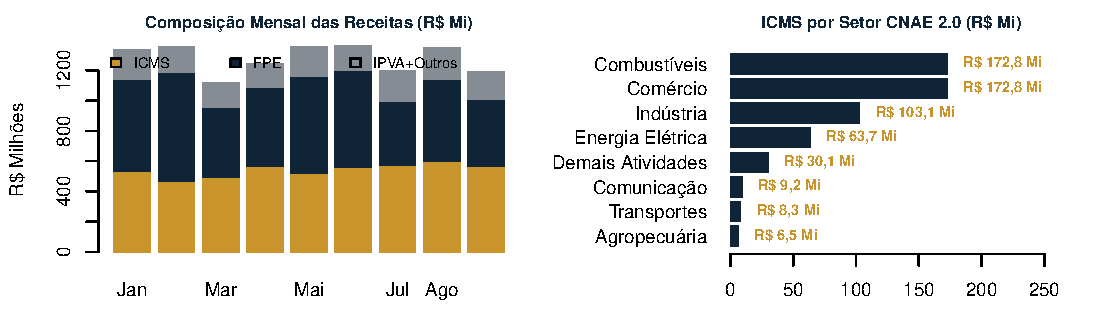
\includegraphics[width=\textwidth]{boletins/build/fig_2026_10_flash_icms.pdf}
\end{center}
\vspace{2pt}
\noindent\begin{minipage}{\textwidth}
{\footnotesize
\noindent\textbf{\textcolor{azulto}{Tabela 1 — Decomposição da Arrecadação de ICMS por Grande Setor e Seção CNAE 2.0 no Tocantins}}\\[3pt]
\begin{tabularx}{\linewidth}{@{}l X r r r r@{}}
\toprule
\rowcolor{azulto} \textcolor{white}{\textbf{Pos.}} & \textcolor{white}{\textbf{Grande Setor / Seção CNAE 2.0}} & \textcolor{white}{\textbf{No Mês}} & \textcolor{white}{\textbf{Part. (\%)}} & \textcolor{white}{\textbf{Acum. Ano}} & \textcolor{white}{\textbf{Var. YoY}} \\
\midrule
1º & Combustíveis e Lubrificantes (Divisão 19 / Seção G CNAE 2.0) & R\$ 172,81 Mi & 30,5\% & R\$ 1.453,80 Mi & +4,29\% \\
2º & Comércio Atacadista e Varejista (Seção G CNAE 2.0) & R\$ 172,77 Mi & 30,5\% & R\$ 1.532,76 Mi & -0,35\% \\
3º & Indústria Geral e Construção (Seções B, C e F CNAE 2.0) & R\$ 103,08 Mi & 18,2\% & R\$ 930,78 Mi & +6,22\% \\
4º & Eletricidade e Gás (Seção D CNAE 2.0) & R\$ 63,73 Mi & 11,2\% & R\$ 481,18 Mi & +19,91\% \\
5º & Demais Serviços e Outras Atividades (Seções I, K-S CNAE 2.0) & R\$ 30,11 Mi & 5,3\% & R\$ 250,70 Mi & -6,62\% \\
6º & Informação e Comunicação (Seção J CNAE 2.0) & R\$ 9,20 Mi & 1,6\% & R\$ 87,42 Mi & -0,47\% \\
7º & Transporte, Armazenagem e Correio (Seção H CNAE 2.0) & R\$ 8,27 Mi & 1,5\% & R\$ 67,73 Mi & +5,64\% \\
8º & Agropecuária (Seção A CNAE 2.0) & R\$ 6,52 Mi & 1,2\% & R\$ 66,59 Mi & -3,88\% \\
\bottomrule
\end{tabularx}
}
\end{minipage}
\vspace{4pt}


% ==============================================================================
% SECAO 2: ANALISE HUMANA E INTERPRETACAO DA EQUIPE
% ==============================================================================
\secaojornal{2. Análise de Conjuntura e Leitura da Equipe}

A evolução recente das receitas estaduais mostra um fortalecimento importante da arrecadação própria do Tocantins via ICMS. A concentração expressiva da receita tributária nos segmentos de Comércio Atacadista, Combustíveis e Comércio Varejista está diretamente ligada à geografia econômica do Estado: como corredor obrigatório de cargas entre o Sul/Sudeste e o Norte/Nordeste, o consumo de óleo diesel e a atividade de distribuição atacadista funcionam como verdadeiros termômetros em tempo real da atividade econômica regional.

\vspace{4pt}

Ao mesmo tempo, a complementaridade entre a arrecadação própria (ICMS e IPVA) e as transferências constitucionais do Fundo de Participação dos Estados (FPE) garante previsibilidade de caixa ao Tesouro Estadual, permitindo a manutenção do cronograma de investimentos públicos em malha viária e serviços essenciais.

% ==============================================================================
% SECAO 3: PERSPECTIVAS E CENARIOS
% ==============================================================================
\secaojornal{3. Perspectivas e Cenários}

Nos próximos meses, a intensificação do transporte da safra e o aquecimento das vendas de fim de ano devem sustentar o crescimento real da receita de ICMS, ampliando o espaço fiscal para o fechamento do exercício orçamentário com equilíbrio nas contas públicas.

\vfill
\noindent{\color{borda}\rule{\textwidth}{0.5pt}}\\[-2pt]
{\scriptsize\textcolor{cinzasuave}{\textbf{Nota Metodológica e Fontes:} Secretaria da Fazenda do Estado do Tocantins (SEFAZ-TO) e Secretaria do Tesouro Nacional (STN). Elaboração: Jornal Econômico do Tocantins. Documento gerado de forma automatizada pelo Sistema Editorial Híbrido (R + LaTeX) do Jornal Econômico do Tocantins.}}

\end{document}
